
%(BEGIN_QUESTION)
% Copyright 2009, Tony R. Kuphaldt, released under the Creative Commons Attribution License (v 1.0)
% This means you may do almost anything with this work of mine, so long as you give me proper credit

Read and outline the ``Proportional Control Action'' subsection of the ``Analog Electronic PID Controllers'' section of the ``Closed-Loop Control'' chapter in your {\it Lessons In Industrial Instrumentation} textbook.  Note the page numbers where important illustrations, photographs, equations, tables, and other relevant details are found.  Prepare to thoughtfully discuss with your instructor and classmates the concepts and examples explored in this reading.

\underbar{file i04267}
%(END_QUESTION)





%(BEGIN_ANSWER)


%(END_ANSWER)





%(BEGIN_NOTES)

The algorithm for a proportional controller is as follows:

$$m = K_p e + b$$

\noindent
Where,

$m$ = Output

$K_p$ = Controller gain (how "aggressive" the controller will be)

$e$ = Error (PV $-$ SP or SP $-$ PV)

$b$ = Bias

\vskip 10pt

A three-opamp ``subtractor'' circuit may be used to calculate error ($e$) from PV and SP.  Gain ($K_p$) is easily implemented using an inverting amplifier with variable feedback, yielding a range of gain values from 0 to far greater than 1.  The bias term ($b$) may be added to the multiplied error term ($K_p e$) using a ``summer'' opamp circuit.

$$\includegraphics[width=15.5cm]{i04267x01.eps}$$








\vskip 20pt \vbox{\hrule \hbox{\strut \vrule{} {\bf Suggestions for Socratic discussion} \vrule} \hrule}

\begin{itemize}
\item{} Explain the operation of the proportional-only analog electronic controller shown in the textbook.
\item{} Explain how the proportional-only analog electronic controller shown in the textbook is able to be switched between {\it direct} and {\it reverse} actions.
\item{} Explain why the DPDT switch shown in the proportional controller circuit is labeled as such (reverse action to the left, direct action to the right).
\item{} Explain why the bias potentiometer is shown powerer by the {\it negative} power supply rail (-V) rather than the positive rail as it is with the setpoint potentiometer.
\item{} Explain how to modify the proportional-only analog electronic controller shown in the textbook to be able to accept a 4-20 mA current signal at the PV input rather than a voltage signal.
\item{} Explain how to modify the proportional-only analog electronic controller shown in the textbook to be able to output a 4-20 mA current signal rather than a voltage signal.
\item{} Suppose the inverting amplifier circuit shown (one opamp, one potentiometer) were modified such that the potentiometer had a greater total resistance.  What effect, if any, would this modification have on the operation of this circuit?
\item{} Perform a ``thought experiment'' with the inverting summer circuit, whereby you propose random voltage signals at each input terminal and analyze all voltage drops and currents in the circuit to calculate the opamp's output voltage.
\item{} Suppose resistor \underbar{\hskip 30pt} fails open in this circuit.  Identify all the effects of this fault, and how you could diagnose it using nothing but a voltmeter.
\item{} Suppose opamp \underbar{\hskip 30pt} fails with a saturated \underbar{\hskip 30pt} output signal.  Identify all the effects of this fault, and how you could diagnose it using nothing but a voltmeter.
\end{itemize}








\vfil \eject

\noindent
{\bf Prep Quiz:}

Identify the component serving as the {\it gain} adjustment in this analog proportional-only controller circuit:

$$\includegraphics[width=15.5cm]{i04267x01.eps}$$


\vfil \eject

\noindent
{\bf Prep Quiz:}

Identify the component serving as the {\it bias} adjustment in this analog proportional-only controller circuit:

$$\includegraphics[width=15.5cm]{i04267x01.eps}$$


\vfil \eject

\noindent
{\bf Prep Quiz:}

Identify the component serving as the {\it forward/reverse} selector in this analog proportional-only controller circuit:

$$\includegraphics[width=15.5cm]{i04267x01.eps}$$


%INDEX% Reading assignment: Lessons In Industrial Instrumentation, closed-loop control (analog electronic PID controllers, proportional action)

%(END_NOTES)


